% This is LLNCS.DEM the demonstration file of
% the LaTeX macro package from Springer-Verlag
% for Lecture Notes in Computer Science,
% version 2.4 for LaTeX2e as of 16. April 2010
%
\documentclass{llncs}
%
\usepackage{makeidx}  % allows for indexgeneration
\usepackage{epsfig}
\usepackage{subfigure}
\usepackage{amssymb}
\usepackage{amstext}
\usepackage{amsmath}
\usepackage{amsthm}
\usepackage{eqparbox}
%
\begin{document}

\frontmatter          % for the preliminaries
%
%
%
\pagestyle{headings}  % switches on printing of running heads
%
%
\title{Reconstruction of Fine Level Geometric Structure From Stereo Pairs in the \\ Underwater Setting}
%
\titlerunning{Fine Level Geometric Structure}  % abbreviated title (for running head)
%                                     also used for the TOC unless
%                                     \toctitle is used
%
\author{Timothy M. Peters\inst{1}\thanks{These authors contributed equally to this work.} \and Erik A. Nelson\inst{1}$^{\star}$ \and \\
Tyler Vitti\inst{1} \and Timothy Gambin\inst{2} \and 
Christopher M. Clark\inst{3} \and Zo\"{e} J. Wood\inst{1}\thanks{This material
is based upon work supported by the National Science Foundation under Grant No.
0966608.}}
%
%
\authorrunning{Peters and Nelson, et al.} % abbreviated author list
%
%%%% list of authors for the TOC (use if author list has to be modified)
\tocauthor{Timothy M. Peters, Erik A. Nelson, Tyler Vitti, Timothy Gambin, Christopher M. Clark, and Zo\"{e} J. Wood}
%
%
%
\institute{California Polytechnic State University, San Luis Obispo CA 93410, USA
\and
University of Malta, ADDRESS HERE
\and
Harvey Mudd College, ADDRESS HERE}
%
\maketitle              % typeset the title of the contribution

\begin{abstract}
The study of underwater structures, such as wells, cisterns, and water storage systems, can be of historical and scientific significance for archeologists. However, access to and study of such sites is often dangerous or infeasible for humans. Underwater micro-ROVs, such as the VideoRay Pro III GTO, can reach and navigate these locations safely while minimizing harm to the site. Prior work has successfully reconstructed geometric models of such underwater structures with the use of sonar measurements. Although effective, sonar has a limited resolution and omits many fine geometric details. In this paper, we present a preliminary solution towards the reconstruction of fine details of organic underwater shapes using stereo vision. These fine details can then be integrated into 3D models reconstructed from sonar to create a more visually accurate model. We present initial results, error measurements, and detailed methodology for future data acquisition.
\keywords{stereoscopic vision, surface reconstruction, projective texture mapping, underwater mapping}
\end{abstract}
%
\section{Introduction}
\noindent Recent research in the field of mobile robotics has demonstrated the creation of 3D maps of settings otherwise inaccessible to humans, such as narrow tunnels and marine caves~\cite{ICEX11,McVicker}. Progress made in Simultaneous Localization and Mapping (SLAM) algorithms, e.g.~\cite{Williams2000,harbor,Fairfield2006}, allow robots to localize themselves and create these maps using input from sonar, infrared, and other scanning sensors. Such maps, or evidence grids, can then be treated as implicit volumes and then used to construct a geometric model of the scanned regions using marching cubes~\cite{Lorensen}. An example of a geometric model of a well used for water storage can be seen in Figure~\ref{fig:wellNoFine}. Unfortunately, equipment limitations, sensor noise, and probabilistic uncertainty in the data acquisition process cause these models to suffer from a loss of fine geometric details. Loss of detail in the scanning process is a problem for end-users, who wish to study these models or use them for educational purposes. In this paper we present a preliminary solution towards the reintroduction of fine details omitted by sonar data into surface reconstructions via the use of two cameras to capture stereo images of underwater surfaces.  The stereo images are processed to produce disparity maps which contain the fine geometric detail of the original surface. The depth information in each disparity map can then be used to enhance the final geometric model.

This project is a part of a larger ongoing project, with the broad goal of mapping and modeling ancient water storage systems, i.e. cisterns, wells and water galleries located in most dwellings on the islands of Malta, Gozo, and Sicily with a micro Remotely Operated Vehicle (ROV)~\cite{White10,ICEX11,McVicker}.  This paper documents the first use of stereo images for fine level geometry reconstruction. The data used in this paper was gathered through a series of underwater deployments in which multiple sonar scans were gathered and fused into a rough map via a SLAM algorithm.  Stereo images were simultaneously captured and later processed to create disparity maps and then fine level geometry. 
%In order to annex this fine geometry to the general models, both the color data and disparity information from the disparity maps are projected onto the geometric model generated from the sonar data via projective texturing. Finally, the geometry contained within the frustums of the projectors in the model is displaced in accordance with the projected disparity maps, preserving the fine details omitted in earlier stages of reconstruction. 
The stages of our approach can be seen in Figure~\ref{fig:systemblock}.

%The results reported in this paper are from preliminary work in a multidisciplinary setting, utilizing aspects of emerging robotics and computer graphics technology. 
%The goal of this work is the generation of a computer model which includes the fine organic features found in underwater storage systems.
This paper outlines the data acquisition and stereo displacement map computation, describes our solution to displacing rough geometry in accordance with a projected disparity map, and illustrates our results on a model using a partial  data set.
%, and presents for future missions. 
%
\begin{figure*}[!ht]
  \vspace{-0.2cm}
  \centering{
     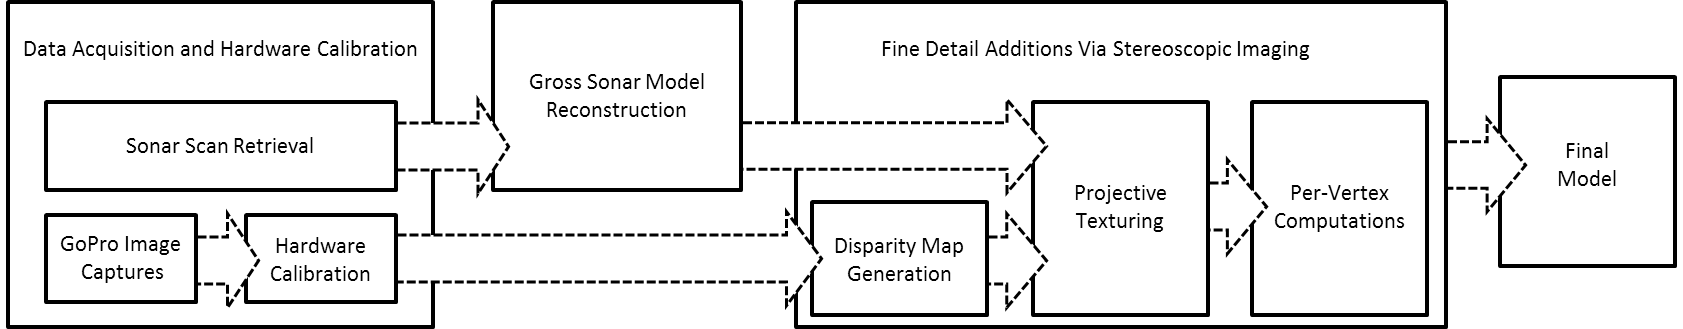
\epsfig{file = pics/systemBlock.png, width = \textwidth}}
  \caption{The pipeline used to add fine details to a sonar generated mesh.}
 \label{fig:systemblock}
\end{figure*}
%
\vspace{-25pt}
\section{Related Work}
\label{sec:related_work}
\noindent This project relies on data acquired from algorithms for mapping with underwater robots~\cite{Williams09,opizarro-2009a,Fairfield2006,Clark2008b}. For a good survey of the core techniques capable of fusing data from multiple sensors, see~\cite{Thrun2005}.
For this project the most relevant  research in underwater robot Simultaneous Localization and Mapping (SLAM) is found in~\cite{Williams2000,harbor,Fairfield2005,Fairfield2006}.

In addition, this work relies on well known algorithms from computer graphics, such as surface extraction from volume data using marching cubes~\cite{Lorensen}, projective texturing and texture mapping~\cite{Williams78castingcurved,Segal}, and the use of vertex shaders to displace existing vertices on the GPU. Work in~\cite{Fairfield:2010} likewise uses marching cubes to create a geometric model of underwater structures from an evidence grid, but uses a far more complex ROV with extensive sensors.
Stereo vision based SLAM algorithms have been used to generate 3D maps of underwater settings~\cite{Mahon:2011,stereo:Roberson,stereo:Aqua}; however, we are using the stereo data to enhance models created from sonar data.

This research relies on related work in the field of stereoscopic data acquisition and disparity map reconstruction~\cite{stereo:scharsteinSzeliski}.
In particular, this work uses the method of~\cite{stereo:zitKan} to generate disparity maps from underwater stereo image pairs.
The work of~\cite{stereo:nalGast} was also explored to compensate for lighting differences, but was found to be ineffective for our setup. 
\vspace{-11pt}
\section{Data Acquisition}
\label{sec:data}
\noindent A VideoRay Pro III GTO micro submersible ROV is utilized in the data acquisition process (Figure~\ref{fig:ROV}). 
%The ROV is deployed into a cistern and guided from a control module above the surface. 
During deployment, the navigator repeatedly rests the ROV on the cistern floor and records a $360^{\circ}$ stationary sonar scan, then the ROV is repositioned for another scan to collect occluded or missing data. 
%The sonar scans must have some overlap to facilitate mosaicing and localization for surface reconstruction, which is taken into consideration when positioning the ROV on the cistern floor. The approximate position and heading of the ROV is recorded before each scan for later use in aligning projectors in the geometric model. The ROV's main video camera is used to position the unit at each location. 
A more complete overview of the sonar data acquisition process can be found in~\cite{ClarkVast}. 
%This collection of sonar scan planes is then used to build a general 3D model~\cite{ICEX11}.

While the sonar scans are being collected, the ROV captures stereo image pairs of the cistern walls. These images are collected using two GoPro HD Hero2 cameras mounted to the front of the ROV, which are synchronized through the 3D Hero System waterproof housing and connector cable. The default domed lenses of the 3D Hero housing distort images taken underwater, so flat lenses were installed to minimize complexity during data processing. The camera unit is unable to be controlled remotely, and instead, each camera is set to capture an image every second. To collect stereo pairs the ROV is maneuvered around the edges of the cistern, pausing every few feet. The ROV is positioned roughly 0.25m to 0.50m from the wall. The images captured at each location are used to create disparity maps.
%
\begin{figure}[!h]
   \vspace{-0.2cm}
   \centering{
      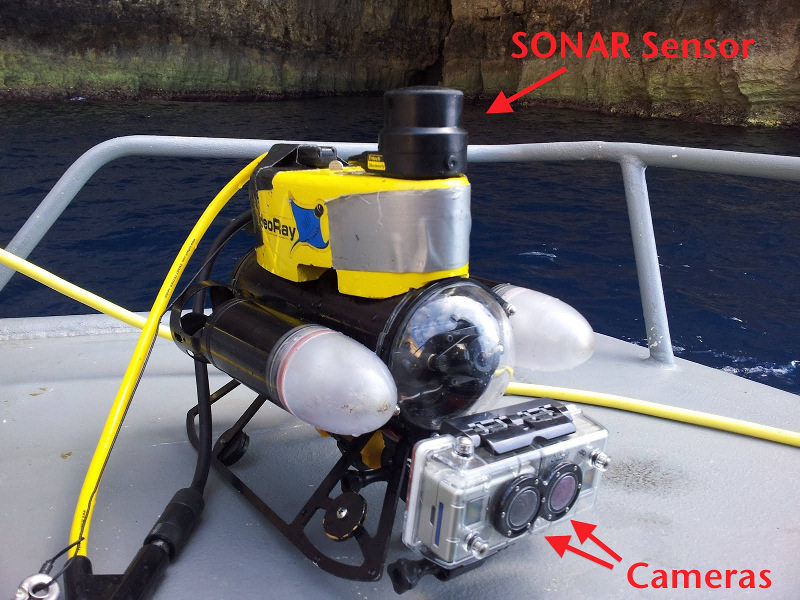
\epsfig{file = pics/ROV.jpg, width = 6cm}}
   \caption{Hardware setup, including a VideoRay Pro III GTO micro ROV, two vertically aligned GoPro Hero2 cameras, and a Tritech SeaSprite sonar sensor.}
  \label{fig:ROV}
 \end{figure}
 %
 \vspace{-25pt}
\paragraph{\textbf{Hardware Calibration:}}
To facilitate the virtual reconstruction of the world it was necessary to calibrate the GoPro cameras.
Both the aspect ratio and the Vertical Field of View (VFOV) need to be calculated to accurately re-project the captured images and disparity maps in the virtual reconstruction.
The cameras were calibrated using the following equations and stereo pairs of a checkered plane submerged in a pool:
\begin{align}
\text{aspect ratio} &= \frac{\text{plane width}}{\text{plane height}} \\
\text{VFOV} &= 2\tan^{-1}\left({\frac{\text{plane height}}{2 \times \text{depth}}}\right)
\end{align}
These two values were used to specify the behavior of projectors, discussed later in Section~\ref{subsec:projectiveTexturing}.

\paragraph{\textbf{Gross sonar Model Reconstruction:}}
\label{sec:reconstruction}
\noindent Prior work is focused on reconstructing general geometric models from evidence maps representing Mediterranean water storage systems (cisterns, wells and water galleries)~\cite{ICEX11,McVicker}. As a pre-process to the algorithms presented here for fine level geometry modeling, the cisterns are mapped using sonar data, which is fused into a two dimensional grid of cells with a likelihood $p_{i,j} \in [0,1]$ of being occupied~\cite{Thrun2005,White10}. This single 2D layer is extruded into a 3D evidence grid and treated as volume data. A polygonal geometric model of the scanned data is constructed via marching cubes, where any cell with $p_{i,j}$ greater than a threshold value is considered an occupied cell and associated with a wall in the model.
We refer the reader to~\cite{ICEX11,McVicker} for more details.

\section{Constructing a more accurate geometric model}
\label{sec:detail}
\noindent Models constructed from evidence grids give a good representation of the gross shape of the underwater system. However, due to challenges in the sonar data acquisition process, these models omit fine geometric details which are important to archaeologists studying the site. See Figure~\ref{fig:wellNoFine} for an example of a well model constructed from sonar data alone. In contrast, Figure~\ref{fig:disparity} shows a photograph of the well wall from inside, where it is clear that fine level details such as rocks and chasms are poorly modeled by the sonar reconstruction.

%The first step towards building fine details into a planar mesh is extracting those details from the original surface. We used stereo vision. 
Fine details were captured in stereo image pairs (left and right images of the same surface), which were used to create disparity maps and record the color data of the surface.
%Due to hardware constraints, our stereo setup is only accurate for determining the distance of objects up to two meters away from the cameras.
%This constraint was not an issue for our purposes, as the ROV was held roughly  from the wall when capturing images.
%EN already said this above
These fine details were integrated back into the existing geometric model by deforming the sonar mesh in accordance with the data stored in the disparity maps, and texturing one of the original images back onto the surface.
There are two challenges at this stage in the process. The first is accurately localizing the ROV with respect to the general model to correctly project the disparity maps onto the model surface. The second is mapping captured depth information onto the existing model.
For the current implementation, we do not include a computational solution to the first challenge. 
Instead, the preliminary results presented in this paper are from a cylindrical well with rotational symmetry, and the user interactively sets the location on the surface from which the image was likely taken in the underwater system.

The second challenge is resolved by using the pixel intensity data stored in the grayscale disparity map to deform the associated vertices.
Light patches of the disparity map pull vertices away from the existing wall, while dark patches push those vertices into the wall.
One of the two stereo images is projected onto the deformed model, adding the color of the original surface to the model. Repeating this procedure for each section of wall produces a finely detailed 3D model of the cistern.
%
\vspace{-10pt}
\begin{figure}[!h]
	\centering
		\subfigure[Well top view]{\label{welltop}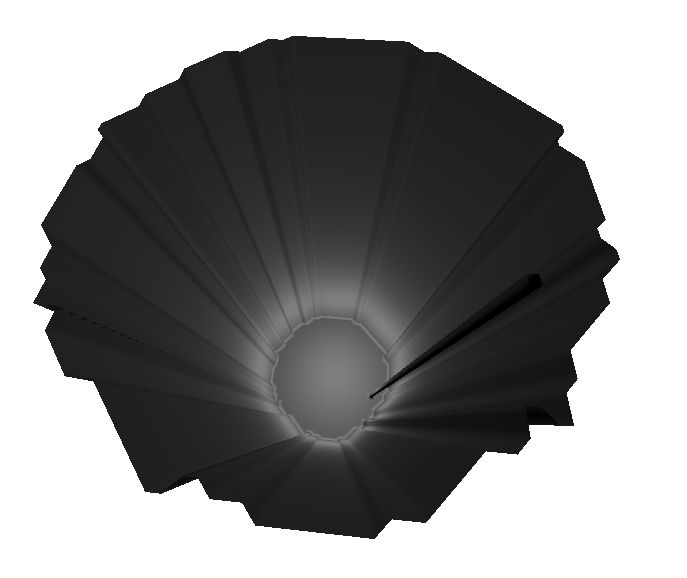
\epsfig{file = pics/cisternTop.png, width = 3.5cm}}
		\quad %space between images
		\subfigure[Well side view]{\label{wellside}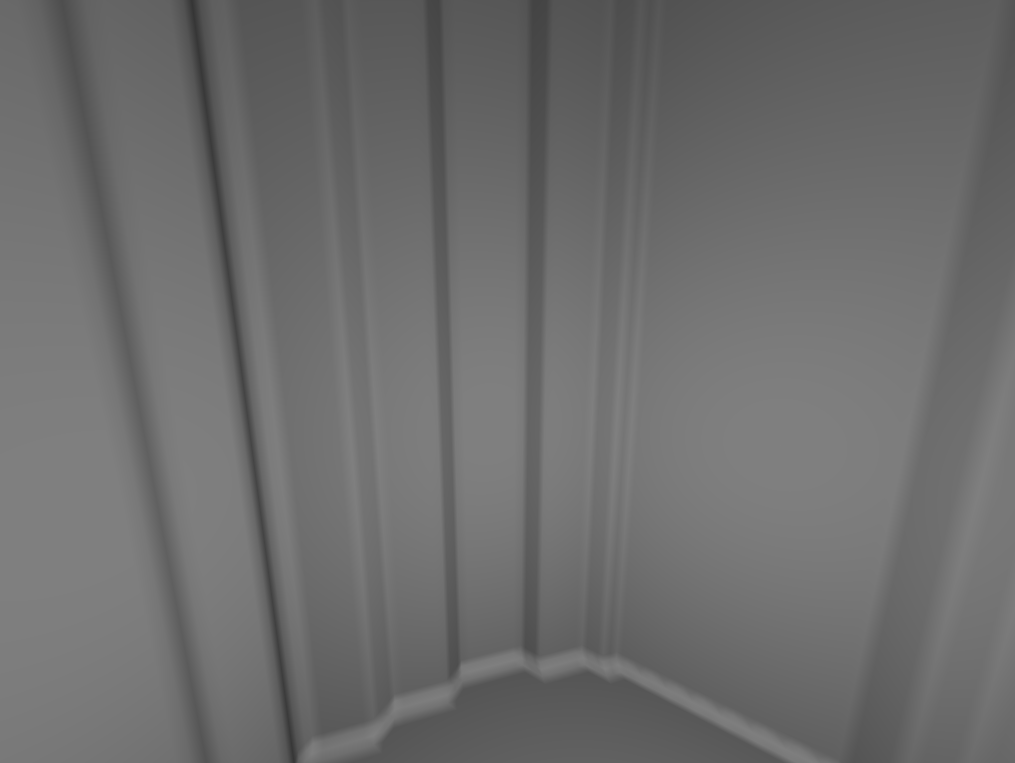
\epsfig{file = pics/cisternWall.png, width = 3.5cm}}
		\caption{Sonar generated well geometry.}
		\label{fig:wellNoFine}
\end{figure}
%
\vspace{-25pt}
\subsection{Disparity Map Generation}
\label{disparityMapGeneration}
\noindent A number of currently existing stereo vision algorithms compare the features of two images to determine the distance between the feature and the camera. However, few of these algorithms are robust enough to handle compressed underwater images of poorly lit rock walls with shallow features. Rocks and bricks, two common features found on cistern walls, have highly repetitive patterns and colors, making feature recognition difficult. In addition, the images captured within the cisterns contain poor lighting and shallow depressions (in comparison to images with large color or depth contrast). After exploring several options, the stereo mapping algorithm described by Zitnick and Kanade in~\cite{stereo:zitKan} was used.

Most stereo-matching algorithms, including Zitnic and Kanade, rely on unique features between images to aid in pixel mapping. Specifically, the algorithm proposed in~\cite{stereo:zitKan} uses a scanning, sliding comparison window to build an initial disparity map. To mitigate the dull landscape, we choose a large initial comparison window with a radius of five pixels. A large window gives a more reliable matching between rock faces because it encompasses more features per pixel. The resulting smoothing effect to the disparity map is acceptable in the given environment.

Lighting was an obstacle to creating good disparity maps. The explored water systems have only a little natural light entering through narrow tunnels, so the imaged surfaces were lit almost exclusively by the ROV's onboard lights.  For which, the ROV had to be within a meter of the walls in order to illuminate features properly. Each camera computes its own exposure time based on the amount of light it received. Some well illuminated features are closer to one camera than the other, producing discrepancies in exposure times between left and right images, (see Figure~\ref{fig:disparity} for an example of this contrast in lighting). We attempted to use the work in \cite{stereo:nalGast} to fix this problem by shifting the image into the HSL color space. This method failed in the presence of water due to a lack of variance in color in the images.

Another underwater challenge is the presence of dirt particles in the images.
The ROV's positioning thrusters often agitate sediment in the water systems. Usually the particles are small enough to be detected as occlusions and removed from the final disparity map.
\begin{figure}[!h]
	\centering
		\subfigure[Left image]{\label{camleft}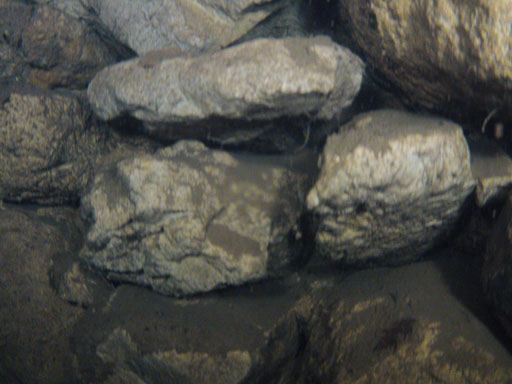
\epsfig{file = pics/372L.jpg, width = 0.3\textwidth}}
		\quad %space between images
		\subfigure[Right image]{\label{camright}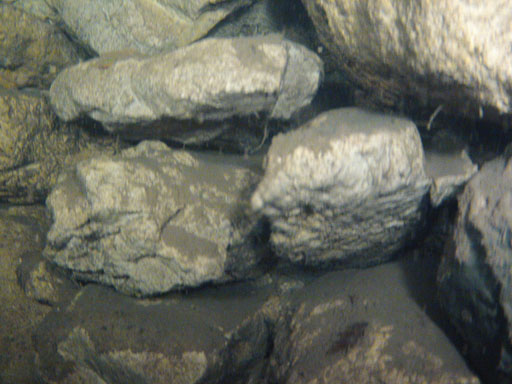
\epsfig{file = pics/372R.jpg, width = 0.3\textwidth}}
		\quad
		\subfigure[Disparity Map]{\label{disparitymap}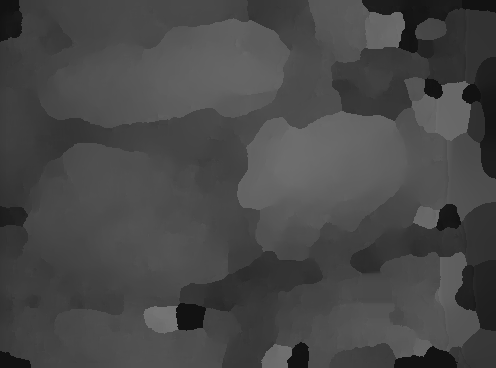
\epsfig{file = pics/372disp.png, width = 0.3\textwidth}}
		\caption{A disparity map generated using the Zitnic Kanade algorithm with initial local support region of (13,13,5), and an iterative support region of (11,11,5).}
		\label{fig:disparity}
\end{figure}
%
\vspace{-25pt}
\paragraph{\textbf{Image Correction:}}
In many stereo mapping algorithms, including Zitnick and Kanade, it is assumed that both images are accurate down to the pixel level. Regrettably, the GoPro cameras used were limited to recording images in the lossy .jpeg format only. To solve this issue we smoothed and shrunk the high resolution .jpeg images taken by the GoPros to produce smaller left and right images that were comparable at the pixel level. For smoothing a simple Gaussian was ineffective because it blurred the edges of the rocks or bricks, removing valuable features from an already feature-scarce image. Instead, an image smoothing tool was used (Photoshop's ``surface smooth''), which preserved edges while still blurring similar color regions. Next a shrinking step was performed on the image to further reduce artifacts (e.g. from 3200 by 2400 to 512 by 384 pixels).
The final size was large enough to preserve the details in the image, while still providing a significant reduction to artifacts.
%Through experimentation, we discovered that the best image detail to process time ratio was obtained by reducing the images by one sixth.   
%Shrinking was performed after smoothing to preserve the maximum amount of detail in the image.

We explored accounting for illumination fade-off, or vignetting, across our image sets, similar to the work in~\cite{stereo:Roberson}. However, due to our close proximity to walls and narrow field of view, de-vignetting had little effect.

%\paragraph{Disparity Mapping}

%Disparity maps were generated using the cooperative, iterative approach described by Zitnick and Kanade~\cite{stereo:zitKan}.
%The basic algorithm is as follows:
%\begin{itemize}
%\item Find the local support region, $L_0$, for each pixel at $(x,y)$ and each disparity, $d$, by using an image intensity comparison function, $\delta$.
%We chose $\delta$ to be a normalized correlation function.
%\begin{equation}
%L_0(x,y,d) = \delta((x,y)_{Left}, (x+d,y)_{Right})
%\end{equation}
%\item Copy the values from the 3D array $L_0$ into a new 3D array, $L_n$.
%\item Let $\Phi(x,y,d)$ be the 3D support region around the pixel $(x,y)$ at $d$, and define the summation of the support region for iteration n as:
%\begin{equation}
%S_n(x,y,d) = \sum_{(x',y',d') \in \Phi(x,y,d)} L_n (x+x', y+y', d+d')
%\end{equation}
%Furthermore, assume that $\Psi(x,y,d)$ is the set of all pixels that map to $(x,y)$ in the left image and $(x+d,y)$ in the right image. 
%Let $\alpha$ be the coefficient of convergence for the values in $L_n(x,y,d)$.  Iterate through the values in $L_n$ updating each value using
%\begin{equation}
%L_{n+1}(x,y,d) = L_n(x,y,d)\left(\frac{S_n(x,y,d)}{\sum\limits_{(x'',y'',d'') \in \Psi(x,y,d)} S_n(x'',y'',d'')} \right)^\alpha 
%\end{equation}
%\item To build the final disparity map, loop through each pixel position $(x,y)$ and award the disparity value $d$ with the highest weight from $L_n(x,y,d)$ as the final value.
%If the best weight for all disparities $d$ for a certain pixel $(x,y)$ is below a predefined threshold, assume the pixel was occluded.
%\end{itemize}

%After the disparity maps were generated, a number of them had obvious errors - small regions of all white and all black. These erroneous regions are fixed by flooring and capping the intensity of the pixels. Pixels that are unreasonably dark simply have their intensity increased to a reasonable minimum correlating to roughly one meter from the camera, while groups of pixels that are too bright are replaced by a linear smoothing of the surrounding pixel values. 

%Using these methods, the computed disparity maps are then used to provide depth values to displace the general geometry created from the sonar data. Figure~\ref{fig:disparity} illustrates a disparity map generated using our implementation.

\paragraph{\textbf{Calibration:}}
The algorithm must be calibrated to create a tuned mapping from a grayscale pixel value to the appropriate vertex offset (distance from the camera to the object) in the virtual reconstruction. To accomplish this, stereo images were taken at right angles to a patterned surface at a number of measured distances. The stereo images were disparity mapped, and the average disparities at the center of each image were used as data points. This set of points, as well as the measured distances from camera to object, were used to determine an exponential relationship between disparity value and physical depth, $D(C_r)$, which is used later in Section~\ref{subsec:displacements}.

\subsection{Projective Texturing}
\label{subsec:projectiveTexturing}
\noindent In order to add fine details to the general mesh created from sonar data, $M_s$, we map the location of the disparity map data onto the global coordinates of the general mesh. Ideally, localization of the ROV's position could be computed and then used to correspond the coordinates of the general mesh and the displacements. With our current hardware, ROV localization is only computed for fixed scans and the ROV's position with respect to the map is unknown for each stereo pair capture. Future work includes using additional hardware such as a Smart Tether to assist in localization, but for our preliminary results, we use projective texturing with a user's input to manually align disparity map and image projections. In general, the onboard camera captures an image of an organic feature in a cistern, and our implementation allows the user to position a projector which casts the image from the same relative position onto the general mesh for displacement. Projective texturing is utilized because of its ability to properly simulate the onboard camera as a point particle with the camera's view frustum modeled as six implicit plane equations (i.e. modeling the camera field of view). Our implementation allows the projection of multiple textures and disparities, building a more detailed colored model as more images and disparities are incorporated.

The combination of projective texturing and stereoscopic imaging enables our system to selectively displace vertices according to the color of a texture-mapped disparity map that is projected onto a surface. These vertices are displaced along the vector leading from their original 3D position in the mesh to the projector (or virtual camera). We used graphics libraries, OpenGL, and OpenGL Shading Language (GLSL) to aid in projective texturing, the latter being used to create shaders - small programs run per-vertex or per-fragment directly on the GPU. The shaders are programmed to selectively alter rendered vertex position (vertex shader) and color (fragment shader).

A projector is simulated by establishing plane equations for a view frustum based on the position and orientation of the ROV's onboard camera when the projected images were captured in a cistern. We define $J = \{j_{1},\dots,j_{N}\}$ to be the set of projectors casting textures onto the gross surface reconstruction. Each projector, $j_{n} = \{j_{n}^{pos}, j_{n}^{look}\}$, is uniquely defined by its position in 3D space, and a look vector orthonormal to the projector's viewport (Figure~\ref{fig:frustum}). All projectors have a pre-calibrated VFOV mimicking the compound VFOV produced by the GoPro camera and waterproof housing lenses, determined in Section~\ref{sec:data}. The ROV is not equipped with roll thrusters, allowing us to ignore the possibility of a tilted camera frustum (i.e. the projector's right facing vector will always lie in the horizontal plane). Implicit plane equations modeling the projector view frustums in the form $Ax + By + Cz + D = 0$ are resolved using the clip space approach, where $\langle A, B, C\rangle$ is the plane's normal vector and  $(x, y, z)$ is a point on the plane. In this approach, plane equations for each projector are computed in homogenous space using the composite $4x4$ modelview projection matrix of the projector, $mvp_n$. 
%See~\cite{vfc} for more information on the projective texturing implementation.

Each vertex, $p_{m}$, is defined by its position in 3D space. The full set of vertices contained in the mesh, $P$, is passed through a view frustum culling filter, yielding a second set containing only those vertices in the frustum volume of one or more projectors, $P^*$ (Figure~\ref{fig:frustum}). Both $P$ and $P^*$ are sent to the shaders for per-vertex displacement computations.
%
\vspace{-10pt}
\begin{figure}[!h]
   \vspace{-0.2cm}
   \centering{
      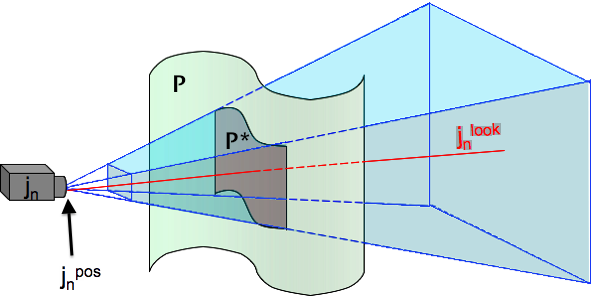
\epsfig{file = pics/frustum.png, width = 5cm}}
   \caption{The vertices intersected by the frustum of the projector are added to $P^*$.}
  \label{fig:frustum}
 \end{figure}
%
\vspace{-25pt}
%EN: not needed
%The implemented projective texturing method naturally produces a second projection facing in the direction negative to $j_{n}^{look}$. To remove the unwanted projections, a simple check was added to the vertex shader which ensures that the texture mapped vertex position has a positive $q$ component.

\subsection{Per-Vertex Displacements}
\label{subsec:displacements}
\noindent A GLSL vertex and fragment shader are used to displace and texture vertices. The vertex shader receives all of the vertices in the mesh, $P$, with vertices lying in the frustum of one or more projectors, $P^*$, marked. The vertex shader also receives a modelview projection matrix ($mvp_n$) for the camera and each projector, projector positions, and texture primitives for the disparity maps from the CPU. The vertex shader displaces vertices one at a time in accordance with the color of the disparity map with respect to the texture-mapped coordinates. Vertices belonging to $P^{*}$ have their position updated. Vertices lying in the frustum of two or more projectors have their displacement vectors blended.

Since the vertex shader is run individually per vertex, it does not have easy access to neighboring vertices. Thus in order to correctly compute normal vectors of the displaced mesh for diffuse shading, the updated position of each vertex must be sent back to the CPU where normals are recomputed for the displaced mesh. Updated normals as well as the displaced mesh are then sent to a fragment shader from the CPU. The displacement vertex shader is only used on the first render.

The fragment shader receives $P$ and $P^{*}$, as well as the camera image texture primitives and the updated normals. The fragment shader maps the camera images onto the vertices in the frustum of each projector. Again, vertices lying in the frustum of two or more projectors have their colors blended. Once an RGB color value has been computed for the vertex, diffuse shading is added to the model using the updated normals.

\paragraph{\textbf{Vertex Displacement:}}
Vertices belonging to $P^{*}$ are displaced along the vector $\vec{b} = j_{n} - p_{m}$ a distance based on the RGB color value, $\vec{C} = \langle C_{r}, C_{b}, C_{g} \rangle$, of the disparity map at the corresponding texture-mapped coordinates, $t_m$. The texture-mapped coordinates of $p_m$, and thus, $\vec{C}$ can be calculated per-vertex using the modelview projection matrix of the projector by
\begin{align}
t_{m} &= p_{m} mvp_{n} \\
\vec{C} &= \langle t_{m\_red}, t_{m\_blue}, t_{m\_green} \rangle
\end{align}
The disparity map is greyscaled such that the disparity value is stored within each of the three members of $\vec{C}$, so only $C_r$ is required for distance computations. The disparity map contains disparity information rather than distance to the wall, so $C_r$ is passed into an exponential equation obtained during calibration, $D(C_r)$, to resolve the true distance to the wall. The world space coordinates of $M_s$ are computed such that one unit in world space is equal to one meter in the cistern, so the value returned from passing $C_r \in [0, 1]$ into the distance function is the true wall distance in meters. With this in mind, vertex displacement proceeds as follows:
\begin{equation}
p_{m}' = \left \{ 
\begin{array}{ll}
p_{m} + (\vec{b} - D(C_r)\hat{b})  & \text{if} \quad p_{m} \in P^{*}\\
p_{m} & \text{otherwise}
\end{array},\right.
\label{eq:displace}
\end{equation}
where $p_{m}'$ is the displaced vertex position. For the results in this paper, we use the calibrated distance function
\begin{equation}
D(C_r) = 0.2179\ln{\left(\frac{C_r}{1.547}\right)}
\label{eq:calibration}
\end{equation}
 \paragraph{\textbf{Projection Blending:}}

%Feel free to remove/edit/use for inspiration
The existence of multiple projectors in the model requires the ability to artfully and accurately overlap and blend projections. 
%Every projection has an equal likelihood of being the ground truth data for a vertex. 
%ZJW I disagree with that statement
Currently, each projection that is applied to a vertex has equal weight upon that vertex's final color and position. Let us assume $J_1$ is the set of all projectors casting a disparity value onto this vertex. Then, expanding on equation~\ref{eq:displace} for $q$ overlapping projections,
\begin{equation}
p_{m}' = \left \{ 
\begin{array}{ll}
p_{m} + \sum\limits_{j \in J_1} \frac{\vec{b} - D(C_r)\hat{b}}{q} & \text{if} \quad p_{m} \in P^{*}\\
p_{m} & \text{otherwise}
\end{array}\right.
\label{eq:displaceBlend}
\end{equation}
Similarly, color values of the texture-mapped final image are equally weighted for overlapping projections to compute the final blend color.
%ZJW just removing for space constraints
%let $C_p$ be the set of all colors projected onto the vertex. Then,

%\begin{equation}
%\vec{C_t} = \sum\limits_{\vec{c} \in C_p} \frac{\vec{c}}{q} 
%\label{eq:colorBlend}
%\end{equation}

%There are other, more complex, methods that could be used to weigh certain projections higher than others, for example by considering distance to the wall and viewing angle, but this simple averaging scheme has worked in practice. 

\section{Results}
\label{sec:results}

\noindent We demonstrate our complete cistern mapping system from a deployment in a rock-walled well in a courtyard in the church, Convento dei Cappuccini, in Council of Carini (near Palermo, Sicily).
A general 3D model shown in Figure~\ref{fig:wellNoFine} was constructed using sonar data from a deployment. The general model is a good representation of the gross shape of the well, but lacks the geometric details of the rocky walls.
Stereo pairs of the inside of the well were captured during deployment for use in generating disparity maps.

Our implementation of the Zitnick and Kanade algorithm was validated against the University of Tsukuba's Multiview Image Database~\cite{stereo:zitKan}, and with the appropriate image filtering and parameter settings (described above) it performed similarly well with rocky underwater cistern images. For example, the image in Figure~\ref{fig:disparity} was generated using an initial support region of size (11,11,5), and an iterative local support region of size (13,13,5). Note that the left and right stereo images have drastically different lighting.
%
%\begin{figure*}[!b]
%   \vspace{-0.2cm}
%   \centering{
%      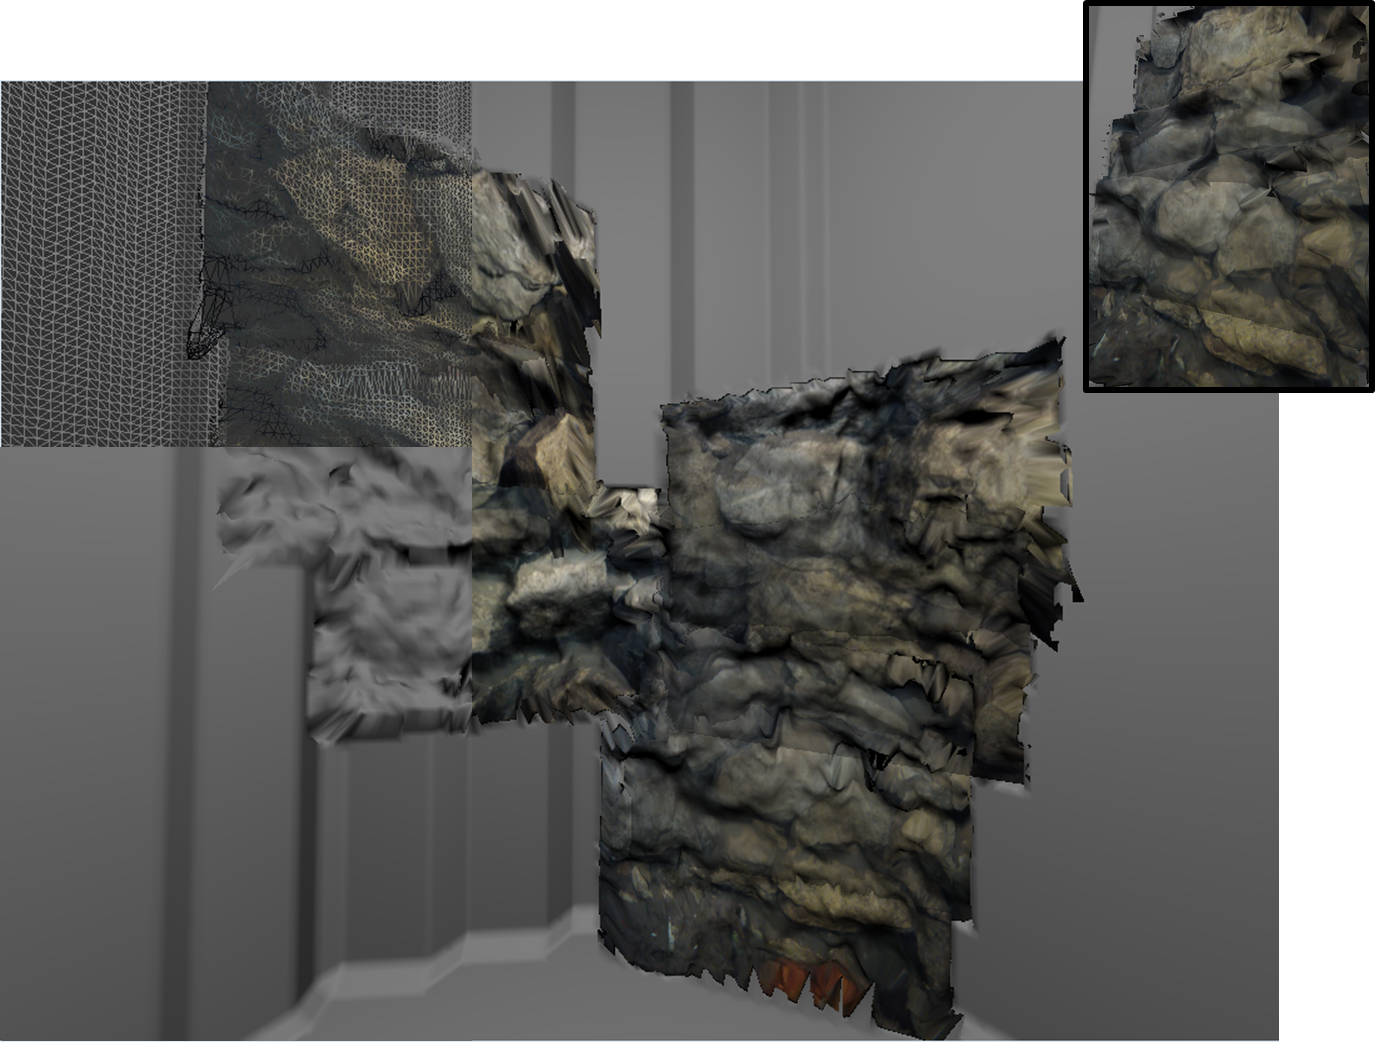
\epsfig{file = pics/400kComposite.png, width = .9\textwidth}}
%   \caption{View of depth and color data mapped onto part of the general mesh. The fine details added by the vertex displacements and recalculated lighting create a better appearance. Image includes inset close-up view.}
%  \label{fig:resultFull}
%\end{figure*}
%
%
%\begin{figure}[!h]
%	\vspace{-0.2cm}
%	\centering
%		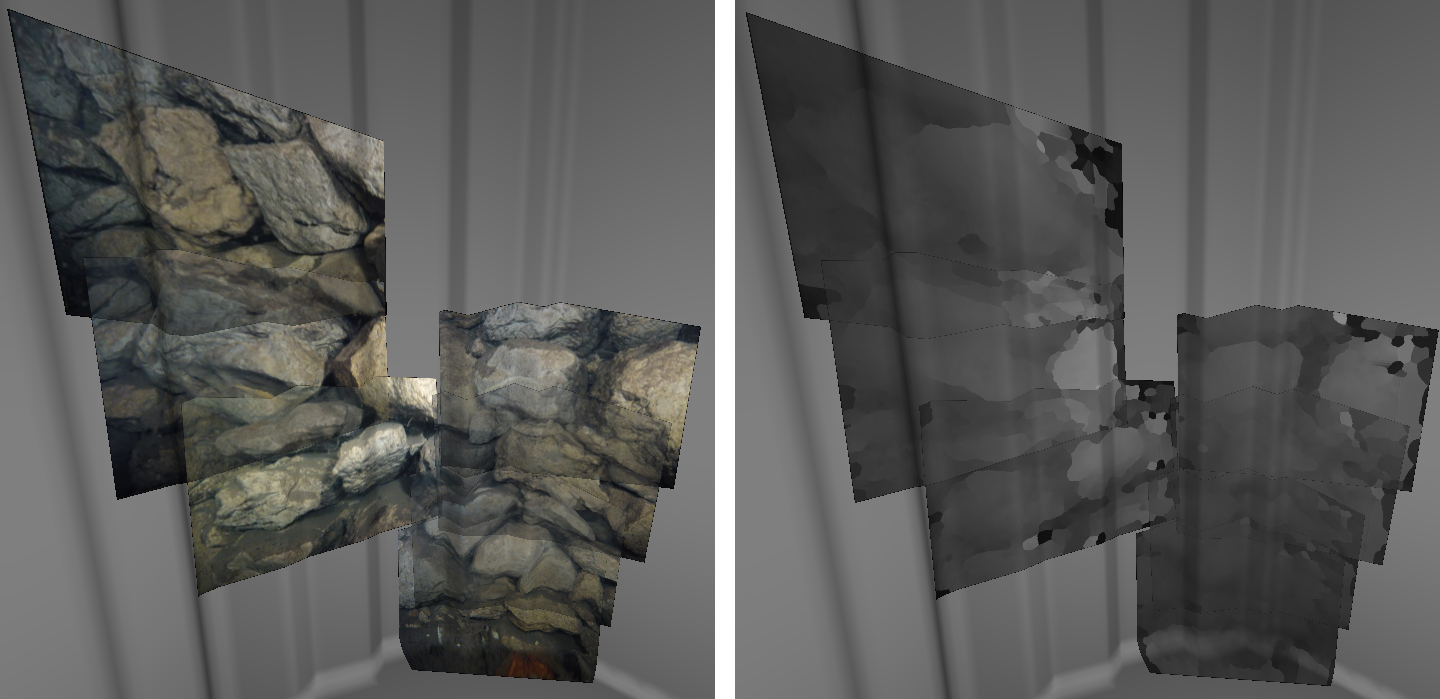
\epsfig{file = pics/NoDisplaceColorDisparity.png, width = 8cm}
%	\caption{Images and disparity maps reprojected as they were captured inside the well with no vertex displacements.}
%	\label{fig:result2}
%\end{figure}
%
%
\begin{figure*}[!t]
	\centering
		\subfigure[Projections without displacements]{\label{fig:result1}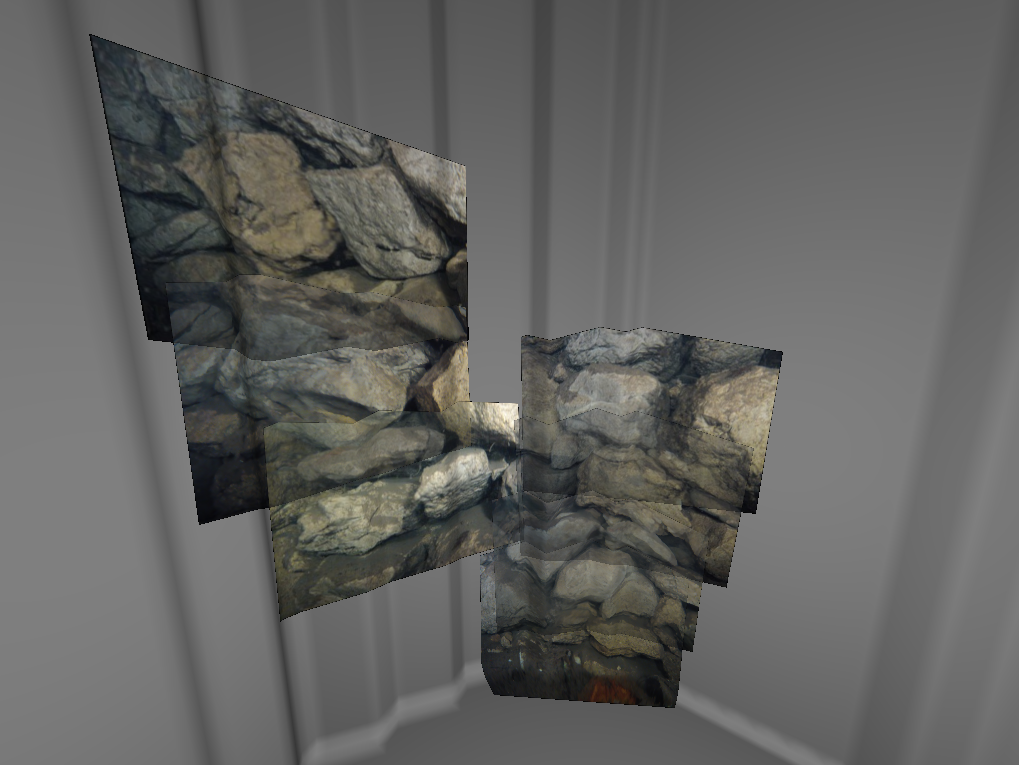
\epsfig{file = pics/finalNoDisplacementNoDisparity2.png, width = 0.45\textwidth}}
		\quad %space between images
		\subfigure[Projections with displacements]{\label{fig:result2}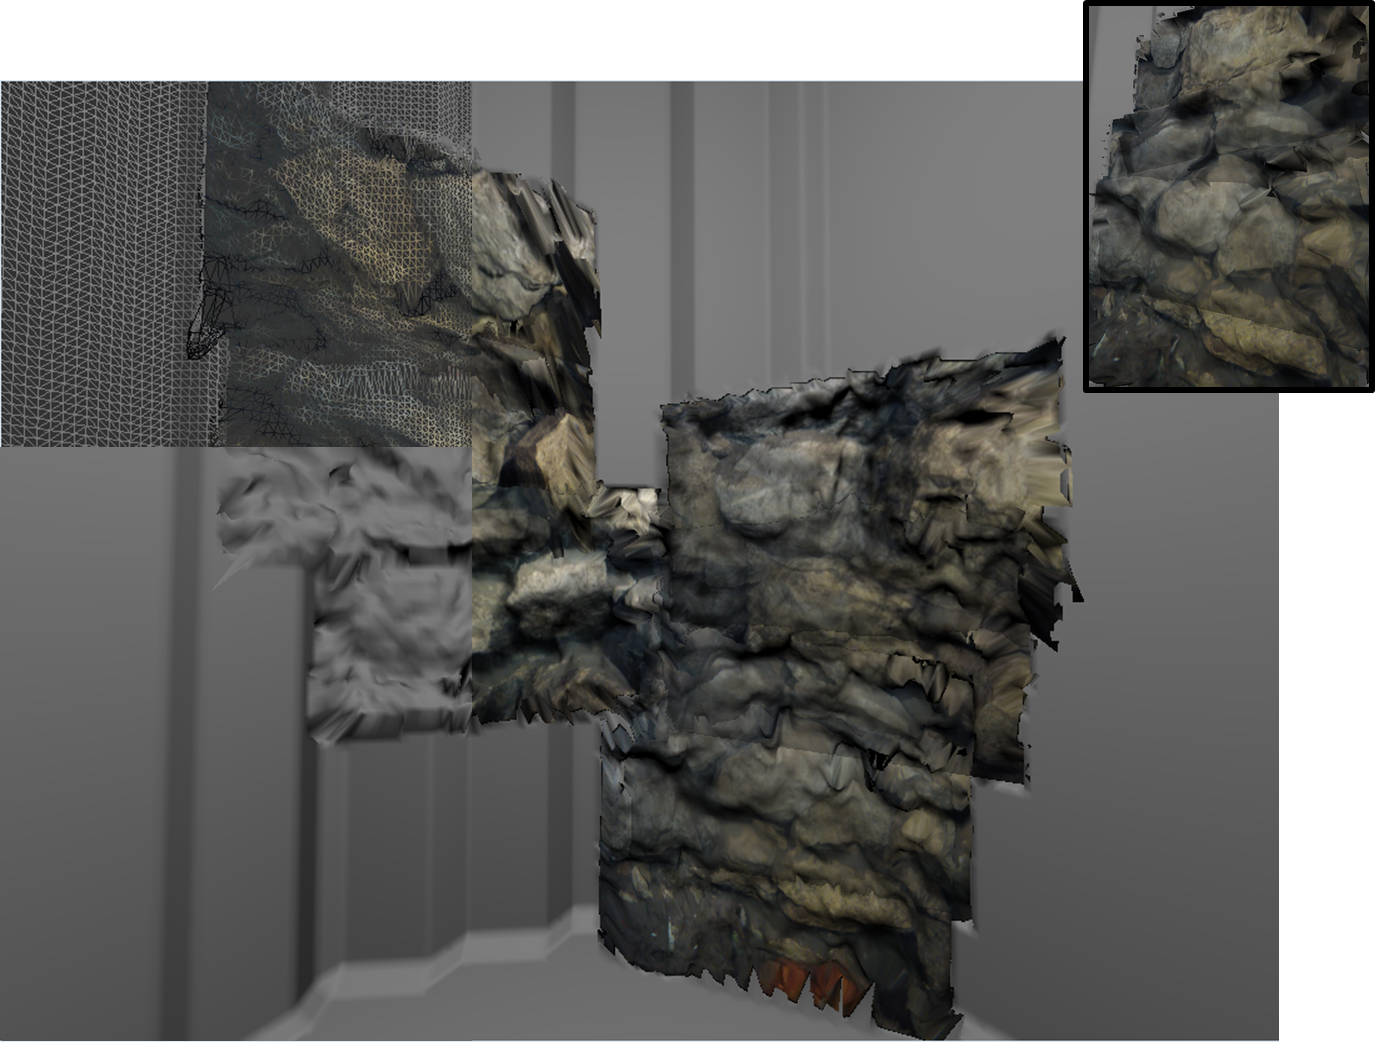
\epsfig{file = pics/400kComposite.png, width = 0.483\textwidth}}
		\caption{View of color data (a), and depth and color data (b) mapped onto part of the general mesh. The fine details added by the vertex displacements and recalculated lighting create a better appearance. Image includes inset close-up view.}
		\label{fig:resultFull}
\end{figure*}
%
Using the geometry from the general mesh constructed from the sonar data, we used projective texturing to display the rock images and disparity maps as they were originally captured at that location as shown in Figure~\ref{fig:result1}. Finally, the disparity maps combined with the surface images were mapped into the well geometry to produce the detailed mesh in Figure~\ref{fig:result2}.

The Cal Poly pool and an angled wooden block were used to validate the accuracy of the displacement algorithm by comparing the measured physical distance from camera to object to $D(C_r)$ determined by the color of a generated disparity map. A wooden block was placed such that it extended from the pool wall at a 45$^{\circ}$ angle, and eight measurements could be taken along its length. Two stereo pairs were captured to gather a total of sixteen data points. The distance from the camera to the pool wall was measured at 0.534$\pm$0.025m for the first disparity map, and 0.520$\pm$0.025m for the second. Physical distance was calculated from the camera to wall distance and measured distances between tick marks along the wooden block using geometry in three dimensions. The error measurements report that the calibration function $D(C_R)$ from~\eqref{eq:calibration} can be used to generate dispalcements accurate to $\pm$0.0325m for camera to object distances between 0.254 and 0.565 meters.

\section{Conclusion and Future Work}
\label{sec:conclusion}
\noindent This paper presents a method of adding geometric details to maps created to represent underwater environments. 
%A general model is acquired from sonar data and mapping~\cite{ICEX11,McVicker,McVicker2}, and we present the addition of fine level details using stereo image data.  
This work is motivated by the desire to better map underwater caverns and cisterns using robotic tools.  We have presented our methodology and hardware for data acquisition, disparity map generation, and incorporation of that disparity data via projective texturing displacements.  We have shown results of a partial reconstruction of a well in Carini, Sicily.

Future enhancements include: the use of higher quality cameras, inclusion of color and more powerful lighting, addition of smart tether for better localization, and enhancement of memory management to process more textures and disparity maps at once.
For future missions, we have learned that since the clearest pictures were taken before the ROV had uplifted sediment from the cistern floor, the ROV should capture all images of the cistern wall before landing. 

In addition, GoPro cameras were a simple, cost-effective, solution to acquire underwater stereo images.
Better cameras would reduce compression artifacts, and ideally images could be captured synchronously.
Alternatively, better lighting, including blue lights, would allow pixel values to be compared in the HSL color space.
It would be useful to explore the integration of this algorithm with SLAM to allow a robot to autonomously image each surface. Finally, we would like to explore algorithms from texture synthesis and apply learning to a small subset of disparity images in order to generalize the small detailed geometry without having to acquire disparity maps of the entire wall (since complete data coverage is a challenge).

%Data collection in future deployments should be performed during a dry weather, as flowing rainwater dirtied the water and reduced image quality for the current data. 

%Unfortunately, that would require a far more complex setup that what we had available at the time of writing.

%ZJW: Please add some suggestion for actual data collection methods as well - re: lighting, positioning ROV, etc.
\begin{thebibliography}{9}
\bibitem{Clark2008b}
Clark, C.~M., Olstad, C., Buhagiar, K., and Gambin, T. (2008).
\newblock Archaeology via underwater robots: Mapping and localization within
  maltese cistern systems.
\newblock In {\em Proc. of the 10th International Conference on Control,
  Automation, Robotics and Vision (ICARCV 08).}

\bibitem{Fairfield:2010}
Fairfield, N., Kantor, G., Jonak, D., and Wettergreen, D. (2010).
\newblock Autonomous exploration and mapping of flooded sinkholes.
\newblock {\em Int. J. Rob. Res.}, 29(6):748--774.

\bibitem{Fairfield2005}
Fairfield, N., Kantor, G., and Wettergreen, D. (2005)).
\newblock Three dimensional evidence grids for {SLAM} in complex underwater
  environments.
\newblock In {\em Proceedings of the 14th International Symposium of Unmanned
  Untethered Submersible Technology (UUST).}

\bibitem{Fairfield2006}
Fairfield, N., Kantor, G., and Wettergreen, D. (2006)).
\newblock Real-time {SLAM} with octree evidence grids for exploration in
  underwater tunnels.
\newblock In {\em Journal of Field Robotics, Vol 24, Issue 1-2, pp. 03-21.}

\bibitem{ICEX11}
Forney, C., Forrester, J., Bagley, B., McVicker, W., White, J., Smith, T.,
  Batryn, J., Gonzalez, A., Lehr, J., Gambin, T., Clark, C.~M., and Wood, Z.~J.
  (2011).
\newblock Surface reconstruction of maltese cisterns using rov sonar data for
  archeological study.
\newblock In {\em Proceedings of the 7th international conference on Advances
  in visual computing - Volume Part I}, ISVC'11, pages 461--471, Berlin,
  Heidelberg. Springer-Verlag.

\bibitem{harbor}
Hernˆndez, E., Ridao, P., Ribas, D., and Batlle, J. (2009).
\newblock Msispic: A probabilistic scan matching algorithm using a mechanical
  scanned imaging sonar.
\newblock In {\em Journal of Physical Agents 3:3Ð11}.

\bibitem{ClarkVast}
Hiranandani, D., White, C., Clark, C., Gambin, T., and Buhagiar, K. (2009).
\newblock Underwater robots with sonar and smart tether for underground cistern
  mapping and exploration.
\newblock In {\em The 10th International Symposium on Virtual Reality,
  Archaeology and Cultural Heritage VAST}.

\bibitem{Lorensen}
Lorensen, W.~E. and Cline, H.~E. (1987).
\newblock Marching cubes: A high resolution {3D} surface construction
  algorithm.
\newblock In {\em Proceedings of the 14th Annual Conference on Computer
  Graphics and interactive Techniques}, pages 163--169.

\bibitem{McVicker}
McVicker, W., Forrester, J., Nelson, E., Gambin, T., Lehr, J., Wood, Z., and
  Clark, C. (2012).
\newblock Mapping and visualizing ancient water storage systems with an rov -
  an approach based on fusing stationary scans within a particle filter.

\bibitem{stereo:nalGast}
Nalpantidis, L. and Gasteratos, A. (2009).
\newblock Stereo vision for robotic applications in the presence of non-ideal
  lighting conditions.
\newblock (28).

\bibitem{opizarro-2009a}
Pizarro, O., Eustice, R.~M., and Singh, H. (2009).
\newblock Large area {3D} reconstructions from underwater optical surveys.
\newblock {\em IEEE Journal of Oceanic Engineering}.
\newblock In Press.

\bibitem{Segal}
Segal, M., Korobkin, C., van Widenfelt, R., Foran, J., and Haeberli, P. (1992).
\newblock Fast shadows and lighting effects using texture mapping.
\newblock In {\em In Computer Graphics (SIGGRAPH Õ92 Proceedings)}.

\bibitem{Thrun2005}
Thrun, S., Burgard, W., and Fox, D. (2005)).
\newblock Probabilistic robotics.
\newblock In {\em MIT Press.}

\bibitem{White10}
White, C., Hiranandani, D., Olstad, C., Buhagiar, K., Gabmin, T., and Clark, C.
  (2010).
\newblock The malta cistern mapping project: Underwater robot mapping and
  localization within ancient tunnel systems.
\newblock In {\em Journal of Field Robotics}.

\bibitem{Williams78castingcurved}
Williams, L. (1978).
\newblock Casting curved shadows on curved surfaces.
\newblock In {\em In Computer Graphics (SIGGRAPH Õ78 Proceedings}, pages
  270--274.

\bibitem{Williams2000}
Williams, S., Newman, P., Dissanayake, G., and Durrant-Whyte, H. (2000)).
\newblock Autonomous underwater simultaneous localization and map building.
\newblock In {\em Proceedings of the 2000 IEEE International Conference.}

\bibitem{Williams09}
Williams, S.~B., Pizarro, O., Jakuba, M., and Barrett, N. (2009).
\newblock {AUV} benthic habitat mapping in {S}outh {E}astern {T}asmania.
\newblock In {\em 7th InternationalConference on Field and Service Robotics}.

\bibitem{stereo:zitKan}
Zitnick, L. and Kanade, T. (1999).
\newblock A cooperative algorithm for stereo matching and occlusion detection.

\bibitem{Mahon:2011}
Mahon, Pizarro, Johnson-Robertson, Friedman, Williams, Henderson. (2011).
\newblock Reconstructing Pavlopetri: Mapping the World's Oldest Submerged Town using Stereo-vision.
\newblock In {\em International Conference on Robotics and Automation}.

\bibitem{stereo:Roberson}
Johnson-Roberson, Matthew and Pizarro, Oscar and Williams, Stefan B. and Mahon, Ian (2010).
\newblock Generation and visualization of large-scale three-dimensional reconstructions from underwater robotic surveys
\newblock In {\em Journal of Field Robotics}.

\bibitem{stereo:scharsteinSzeliski}
Scharstein, Daniel and Szeliski, Richard (1998).
\newblock Stereo Matching with Nonlinear Diffusion
\newblock In {\em International Journal of Computer Vision}.

\bibitem{stereo:Aqua}
Georgiades, C., German, A., Hogue, A., Liu, H., Prahacs, C., Ripsman, A., Sim, R., Torres, L.-A., Zhang, P., Buehler, M., Dudek, G., Jenkin, M., Milios, E. (2004)
\newblock AQUA: An Aquatic Walking Robot 
\newblock In {\em IEEE/RSJ International Conference on Intelligent Robots and Systems}
\end{thebibliography}
\end{document}
